

\begin{comment}
\begin{figure}
\centering
\includegraphics[clip, trim=5.5cm 19cm 5.5cm 6cm, width=0.3\textwidth]{figures/strategy1}
\caption{Evaluation methodology to answer RQ1} 
\label{fig:strategy1}
\end{figure}

\begin{figure}
\centering
\includegraphics[clip, trim=4.5cm 16.5cm 5.5cm 6.5cm, width=0.3\textwidth]{figures/strategy2}
\caption{Evaluation methodology to answer RQ2} 
\label{fig:strategy2}
\end{figure}
\end{comment}

%Furthermore, in software development projects, some traditional programmers might want to practice with code in a traditional way and some MDE developers may prefer working with models. Therefore, it is necessary to compare the development/maintenance cost between the two practices by comparing the number of steps needed to do the same action. 


\subsection{Reversing generated code}
\label{subsec:exp1}
%\tb{RQ1}: A state machine \ttt{sm} is used for generating the front-end code. The latter is reversed engineered to produce another state machine \ttt{sm'}. Are \ttt{sm} and \ttt{sm'} identical? In other words: whether the front-end code generated from USMs model can be used for reconstructing the original model. This question is related to the \ti{GETPUT} law defined in \cite{foster_combinators_2007}.

\begin{comment}
\begin{figure}
	\centering
	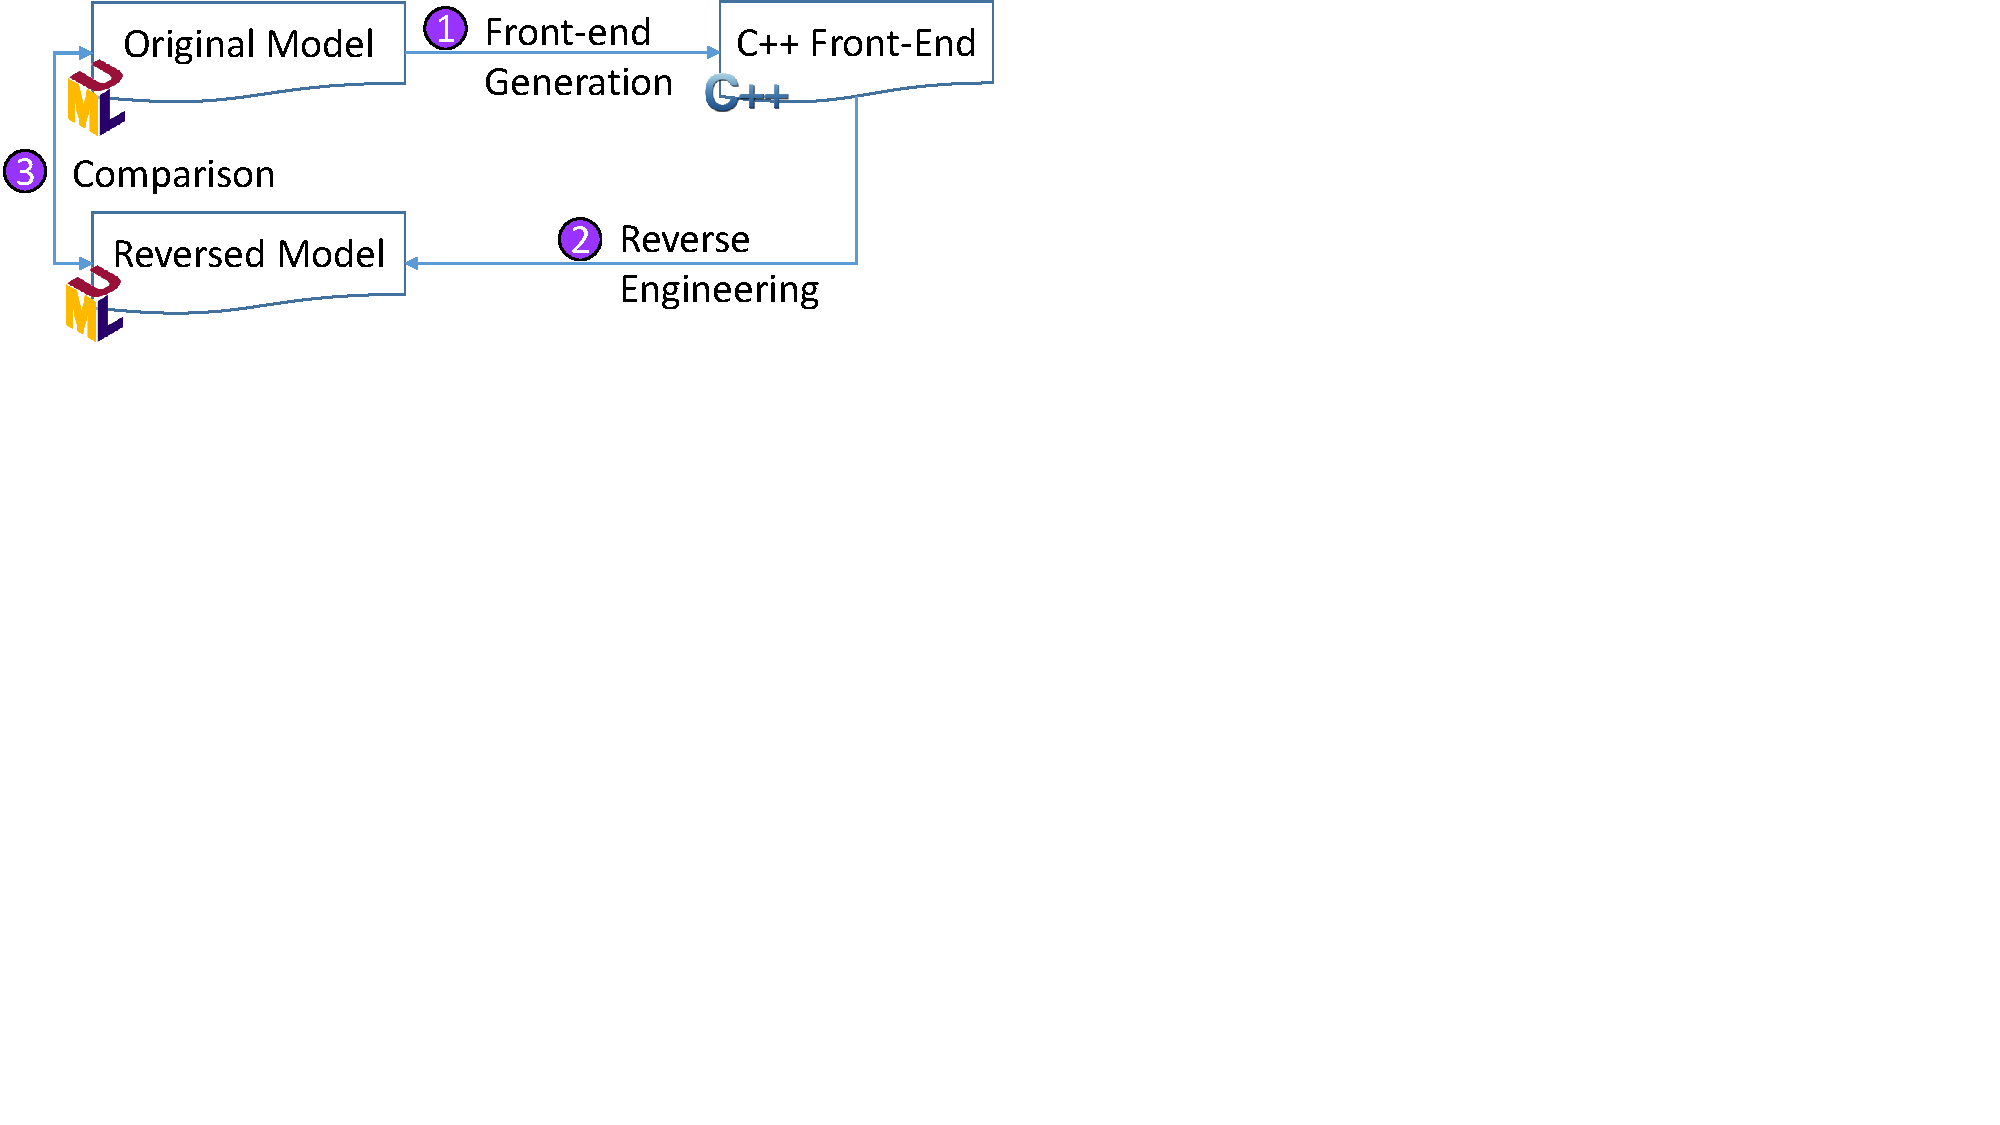
\includegraphics[clip, trim=0cm 13.1cm 16.2cm 0cm, width=\columnwidth]{figures/rteevaluation}
	\caption{Evaluation methodology to answer RQ1} 
	\label{fig:EvaluationStrategyBoth}
\end{figure}
\end{comment}

%This experiment is targeting \tb{RQ1}. 
Fig. \ref{fig:rq1-2evaluation} (a) shows the experimental methodology to answer \tb{RQ1}. 
The procedure for this experiment, for each original UML model containing a state machine, consists of 3 steps: (1) \tb{C++ front-end code} is generated from an \tb{original model}; (2) the \tb{C++ front-end code} is reverse engineered to a \tb{reversed model}; and (3) the \tb{reversed model} is then compared to the \tb{original model}.


\begin{comment}
\begin{description}[\footnotesize]
	\item[Step 1] \ttt{C++ front-end code} is generated from an \ttt{original model}.
	
	\item[Step 2] The \ttt{C++ front-end code} is reverse engineered to a \ttt{reversed model}
	
	\item[Step 3] The \ttt{reversed model} is then compared to the \ttt{original model}.
\end{description}
\end{comment}

%(1) C++ front-end code is generated from an \tb{original model}, (2) the generated code is reverse engineered to a \tb{reversed model}, and (3) the the is then compared to the \tb{original state machine}.% by using information of USM such as the numbers of states and transitions. 

We developed a configurable generator to derive random models. 
%are automatically generated by a configurable model generator. 
The configuration information consists of an active class and its state machine behavior with desired average numbers of vertexes, transitions, and events. 
%For each model, an class and its behavior described by a USM are generated. 
Each USM contains 100 vertices , more than 234 transitions, more than 50 events. 
%The number of lines of generated C++ code for each machine is around 13500. Names of the generated states are different. 
%An initial pseudo state and a final state are generated for each composite state and containing state machine. 
%Other elements such as call events, time events, transition/entry/exit actions and guards are generated with a desired configuration. 
%For each generated call event, an operation is generated in the context class which is also generated. 
%The duration is generated for each time event. 

\begin{comment}
\begin{table}
\centering
\caption{Set-up information for model generation}
\label{table:setup}
\begin{tabular}{|l|l|}
\hline
\rowcolor{Gray}
Description                                     & Value            \\ \hline
%Number of generated states                      & 80               \\ \hline
%Number of generated transitions                 & \textgreater 234 \\ \hline
Probability of having an event for transition   & 0.8              \\ \hline
Probability of having CallEvent for transition  & 0.7              \\ \hline
Probability of having an entry/exit action for state & 0.7              \\ \hline
Probability of having a transition action and guard       & 0.7              \\ \hline
\end{tabular}
\end{table}
\end{comment}

%The set up information for the USM generation is shown in Table \ref{table:setup}. 

\begin{comment}
\begin{table}
\centering
\caption{Three of model results of generation and reverse: Abbreviations are atomic states (AS), composite states (CS), transitions (T), call events (CE), time events (TE)}
\label{table:law1-resultat}
\begin{tabular}{|l|l|l|l|l|l|l|}
\hline
\rowcolor{Gray}
Test ID & AS & CS & T & CE & TE & Is reverse correct? \\ \hline
1       & 47 & 33 & 234 & 145 & 40 & Yes                 \\ \hline
2       & 42 & 38 & 239 & 145 & 36 & Yes                 \\ \hline
%3       & 43 & 37 & 238 & Yes                 \\ \hline
..      & .. & .. & .. & .. & .. & Yes                 \\ \hline
300       & 41 & 39 &240 & 142 & 37 & Yes                 \\ \hline
\end{tabular}
\end{table}
 \end{coment}
 
\begin{comment}
\begin{table*}[]
\centering
\caption{MODEL RESULTS OF GENERATION AND REVERSE}
\label{table:law1-resultat}
\begin{tabular}{|l|l|l|l|l|l|l|l|l|l|l|l|l|l|}
\hline
\rowcolor{Gray}
Test ID & AS & CS & D  & T   & EA & ExA & TA  & CE  & TE & G   & I  &    & Is reverse correct? \\ \hline
1       & 47 & 33 & 8  & 234 & 53 & 50  & 149 & 145 & 40 & 147 & 34 & 25 & Yes                 \\ \hline
2       & 42 & 38 & 8  & 239 & 52 & 59  & 165 & 145 & 36 & 133 & 39 & 31 & Yes                 \\ \hline
3       & 43 & 37 & 7  & 238 & 54 & 59  & 159 & 141 & 34 & 145 & 38 & 28 & Yes                 \\ \hline
..      & .. & .. & .. & ..  & .. & ..  & ..  & ..  & .. & ..  & .. & .. & Yes                 \\ \hline
300       & 41 & 39 & 10 & 240 & 56 & 55  & 165 & 142 & 37 & 151 & 40 & 33 & Yes                 \\ \hline
\end{tabular}
\end{table*}
\end{comment}

%Table  \ref{table:law1-resultat} shows the number of each type of elements in the randomly generated model, including the comparison results, for 3 of the 200 models created by the generator. We limited ourselves to 200 models for practical reasons

%Table \ref{table:law1-resultat} shows the number of several types of elements in the generated models, including the comparison results, for 3 of the 
300 radom models are produced by the generator. 
We limited ourselves to 300 models for practical reasons. 
No differences were found during model comparison. 
The results of this experiment show that the RAOES can successfully do C++ front-end code generation from state machines and reverse. 

%\input{sections/changepropagation}

%\input{sections/timecomplexity}

%
\subsection{Semantic conformance of runtime execution}
\label{subsec:exp2}
\paragraph{Bisimulation for semantic-conformance}
To evaluate the semantic conformance of runtime execution of generated code, we use a set of examples provided by Moka \cite{moka}. Moka is a model execution engine offering Precise Semantics of UML Composite Structures \cite{OMG2015}. Fig. \ref{fig:semanticconformance} shows our method. We first use our code generator to generate code (Step (1)) from the Moka example set. Step (2) simulates the examples by using Moka to extract the sequence (\ti{SimTraces}) of observed traces including executed actions. The sequence (\ti{RTTraces}) of traces is also obtained by the runtime execution of the code generated from the same state machine in a Step (3). The generated code is semantic-conformant if the sequences of traces are the same for both of the state machine and generated code \cite{Blech2005}. The current version of Moka does not support simulation for \ti{TimeEvent} and history pseudo states, we therefore leave experiments for \ti{TimeEvent} as future work.

For example, Fig. \ref{fig:autotransition} (a) shows a USM example with triggerless transitions (\ti{autotransitions}) \ti{T3}. 
The USM contains two states, \ti{Waiting}, which is the initial state, and \ti{Incrementing}, which increases an integer number from 0 to 5 by using the effect of \ti{T3}. The latter also has a guard checking whether the number is less than 5.
The increase is executed after the USM receives an event named \ti{start} to transition the initial state \ti{Waiting} to \ti{Incrementing}. 
Suppose that executions of the effects of \ti{T3} and \ti{T4} produce traces \ti{<T3>} and \ti{<T4>} (by using MOKA, e.g.), respectively. 
Due to the guard of \ti{T3}, the effect of \ti{T3} is executed five times followed by an execution of the effect of \ti{T4}.
After the completion of the USM, the obtained sequence of traces
is \ti{<T3><T3><T3><T3><T3><T4>} (since the \ti{Incrementing} state does not have an \ti{entry}, \ti{exit}, or a \ti{doActivity}, only the transition effect \ti{T3} produces traces). 
The sequence \ti{RTTraces} obtained by the runtime execution %of the code generated from this USM 
must be equivalent. 
\ti{RTTraces} is obtained by simply printing logging information for each action (effect).

Within our scope as previously defined 30 examples of the Moka example set are tested. \ti{SimTraces} and \ti{RTTraces} for each case are the same. 
This indicates that, within our study scope, the runtime execution of code generated by our generator can produce traces semantically equivalent to those obtained via simulation. 


After experimenting with our code generator, we compare our results to the observed traces obtained by executing code generated 
%by IBM Rhapsody \cite{ibm_rhapsody} and 
Umple \cite{Badreddin2014}. 
We find that the obtained traces in case of 
%IBM Rhapsody and 
Umple are not UML-compliant in triggerless transitions and some cases of event processing.
Specifically, for the example in Fig. \ref{fig:autotransition} (a), 
code generated by Umple only produces \ti{<T3>} as the trace sequence. 
Umple does not support events which are accepted by sub-states and the corresponding composite state as in Fig. \ref{fig:autotransition} (b) in which both \ti{S1} and \ti{S21} accept the event \ti{Continue}.
%Rhapsody does not support self-triggerless transitions as in Fig. \ref{fig:autotransition} and its support for processing events is not totally semantically correct. 
As the processing event example in Fig. \ref{fig:autotransition} (b), assuming that there is an event \ti{Continue} incoming to the state machine which has a current configuration \ti{(S1, S21)} as current active states. While, according to the UML specification, the incoming event should be processed by the inner states of the active composite/concurrent state if the inner states accept it, otherwise the parent state does. Therefore, the next configuration should be \ti{(S1, final state)} and the \ti{T22Effect} effect of the transition \ti{T22} should be executed. %But in case of Rhapsody the next configuration is \ti{End}.   


\begin{figure}
\centering
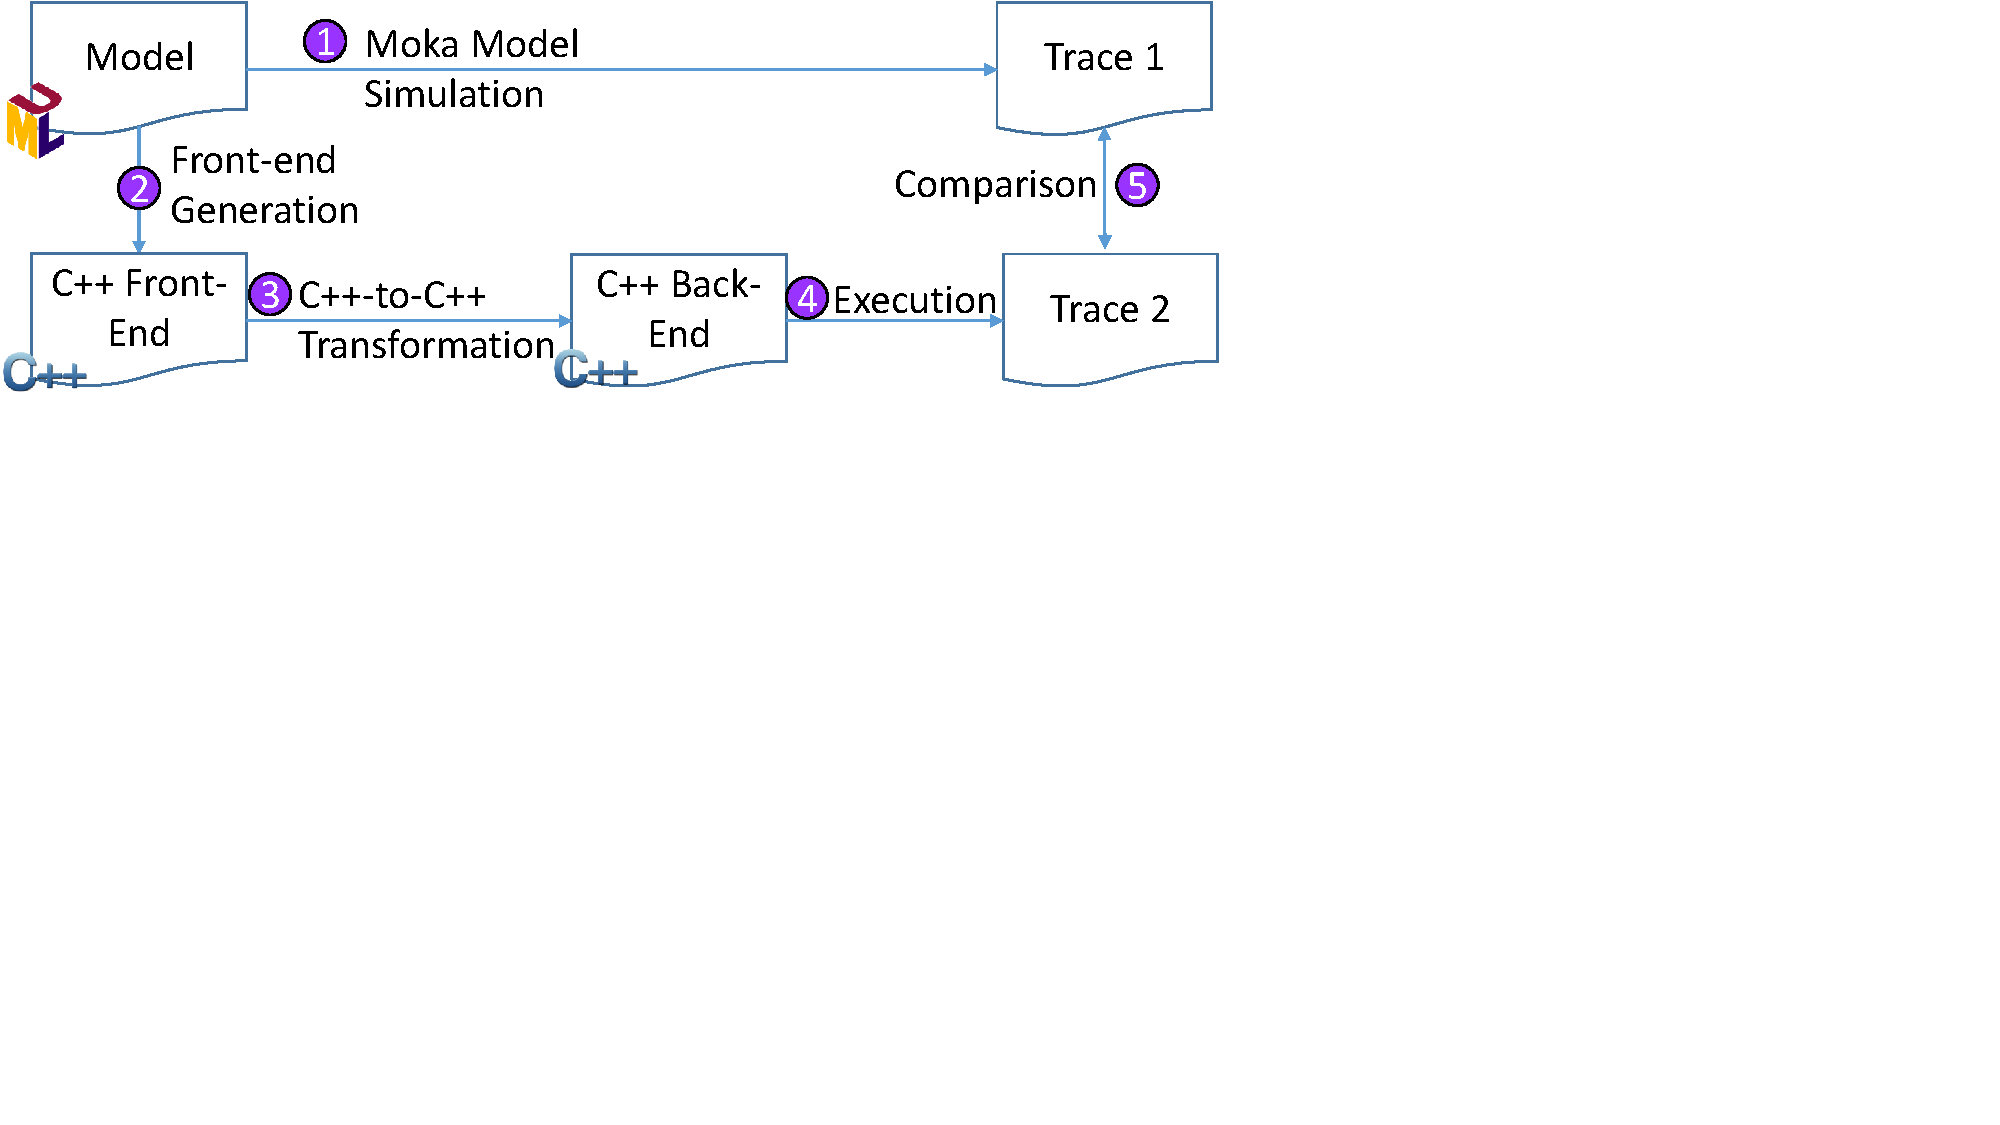
\includegraphics[clip, trim=0.2cm 8.6cm 19.4cm 6.9cm, width=0.8\columnwidth]{figures/semanticconformance.pdf}
\caption{Semantic conformance evaluation methodology} 
\label{fig:semanticconformance}
\end{figure}

\begin{figure}
\centering
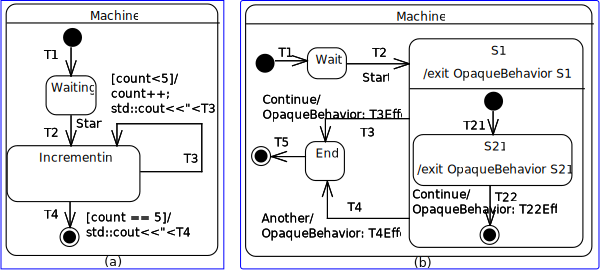
\includegraphics[clip, trim=0cm 0cm 0cm 0cm, width=\columnwidth]{figures/Deferred004Revised}
\caption{Self-triggerless transition and event processing example} 
\label{fig:autotransition}
\end{figure}



\begin{comment}
\begin{figure}
\centering
\includegraphics[clip, trim=0.25cm 0.25cm 0.25cm 0.25cm, width=0.9\columnwidth]{figures/Deferred004}
\caption{Event processing example} 
\label{fig:Deferred}
\end{figure}


\begin{figure*}
\centering
\includegraphics[width=1.5\columnwidth]{figures/ex}
\caption{Self-triggerless transition (a) and event processing (b) examples} 
\label{fig:ex}
\end{figure*}
\end{comment}

\paragraph{Finite state machine}
In addition to the experiment using MOKA, we evaluate the semantic-conformance by using deterministic finite state machines (FSMs). The latter is a mathematical model of computation and also a simplified version of UML state machine. In this experiment, we use FSMs for recognizing input symbols. Each FSM contains many atomic states. The active state of the FSM can be changed following the acceptance of an input symbol. Fig. \ref{fig:fsm} shows our method to experiment. For each FSM, we create an equivalent USM. Each input symbol of the FSM is considered as an event of the USM. We use the FSM simulator in \cite{fsmsim} to generate and simulate FSMs. For each FSM, a list of observed states is recorded as output (\ti{out1}) of the simulation for each symbol list. The latter is also the input of the generated code runtime execution of the equivalent USM which produces an output \ti{out2}. We then compare \ti{out1} and \ti{out2}.

We limit the number of FSMs to 20 and the number of symbol list for each FSM to 30 for practical concerns. 600 sequences of states obtained by the simulation and a same number of sequences taken by the runtime execution are respectively compared and found being equal. This results that our code generation approach can produce semantic-conformant code in case of FSM.

\begin{figure}
	\centering
	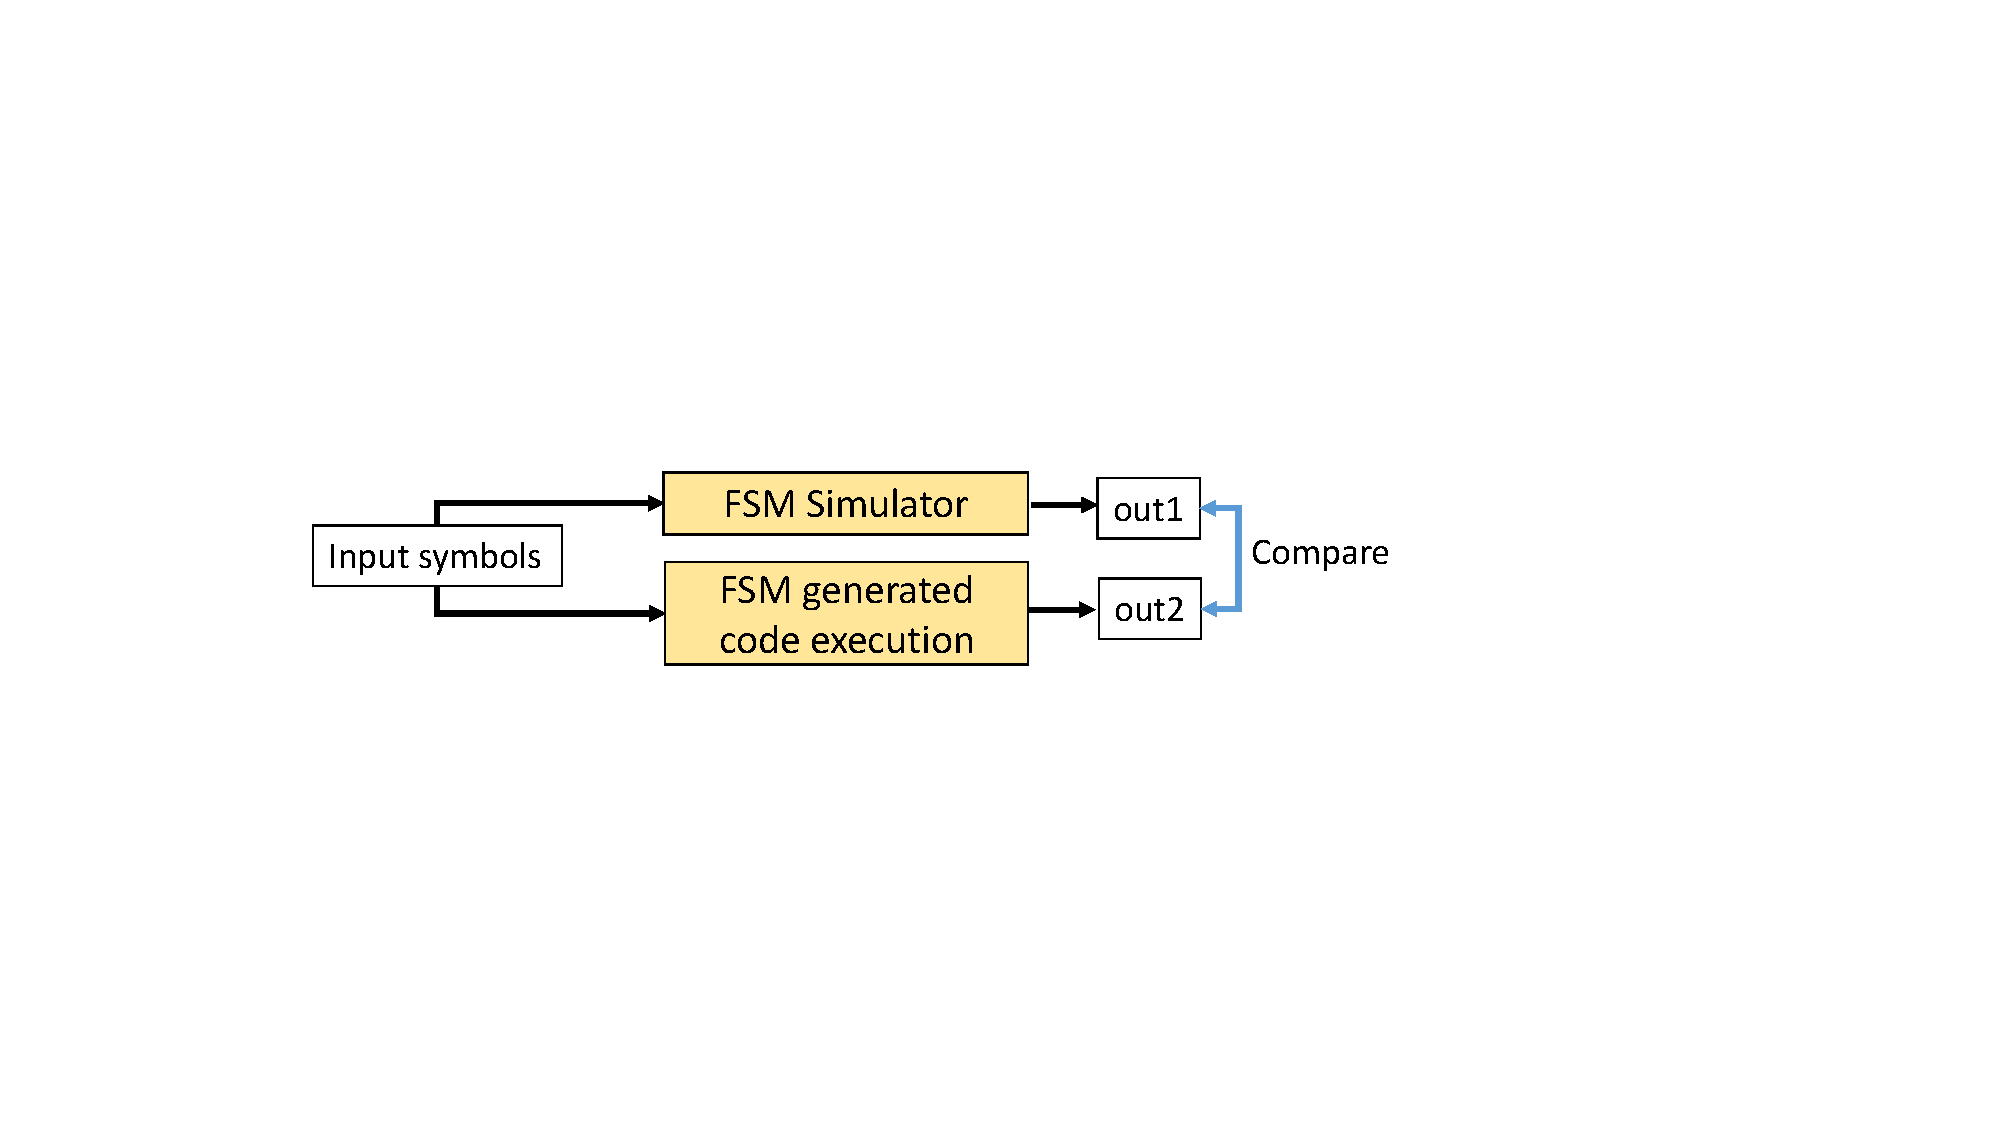
\includegraphics[clip, trim=4.5cm 7.6cm 10.25cm 8.0cm, width=0.85\columnwidth]{figures/fsm}
	\caption{FSM experiment method} 
	\label{fig:fsm}
\end{figure}


%\paragraph{Comparison with IBM Rhapsody}

%\input{sections/developmentcost}